% see A1.4
\chapter{Planen} \label{ch:plan}

Die Zeitplanung wird in der Abbildung \ref{fig:timeplan} oberhalb gezeigt. Die restlichen Aspekte der Planung sind in diesem Kapitel dokumentiert.

\section{Datenmodell}

\subsection{Entity-relationship Diagramm}

Das Entity-relationship Diagramm \ref{fig:erd} zeigt alle für diese PA notwendigen Entitäten und deren Verhältnis zueinander. Die Felder
der einzelnen Tabellen können in der Planungsphase noch nicht vollumfänglich definiert werden und werden höchstwahrscheinlich in einzelnen Fällen während der Realisierungsphase
erweitert. Das Grundkonzept und die Assoziationen zwischen den verschiedenen Entitäten bleiben allerdings gleich.

\begin{figure}[H]
    \centering
    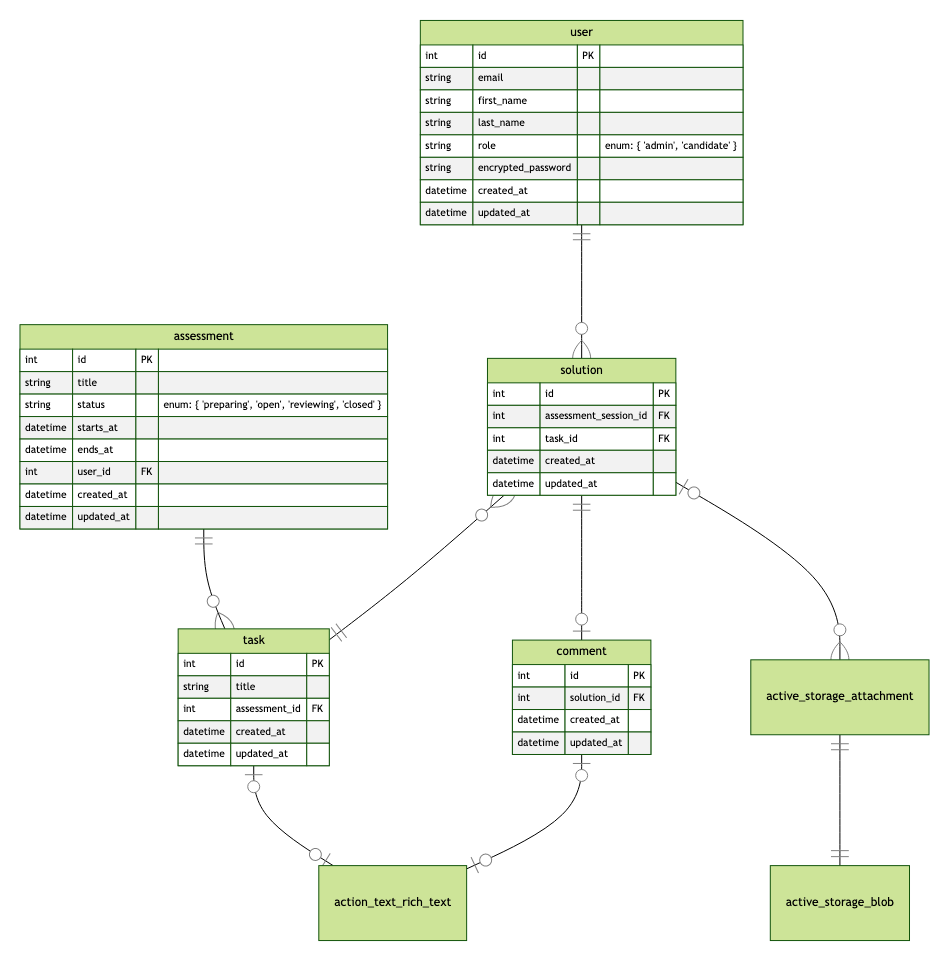
\includegraphics[height=15.25cm]{images/diagrams/entity-relation.png}
    \caption{\label{fig:erd}Entity-relationship Diagramm}
\end{figure}

\newpage

Die drei Entitäten \emph{active\_storage\_attachment}, \emph{active\_storage\_blob} und \emph{action\_text\_rich\_text} werden automatisch durch das
Framework generiert und sollen in diesem Diagramm zum besseren Verständnis des Gesamtkonzeptes beitragen. In der Praxis wird man mit diesen Tabellen direkt kaum etwas zu tun haben.
Diese werden von den zwei gems ActiveStorage und ActionText verwendet, welche das Einbinden von formatierten Textinhalten und Dateiuploads ermöglichen.

Sowohl der Zustand (State) von einem \emph{assessment} als auch die Benutzerrolle von einem \emph{user} wird in Form von einem \gls{enum} abgebildet. Dabei ist zu beachten, dass es in der Praxis kein Database-Level Enum sein wird,
sondern der Wert in Form eines Strings in der Datenbank gespeichert werden soll. Der Constraint wird dann auf Application-Level durchgesetzt. Das ist ein ActiveRecord Standard und ermöglicht eine höhere Flexibilität und Erweiterbarkeit.
Ausserdem werden nicht alle Akteure aus \ref{tab:participants} in Form von Benutzerrollen in der \emph{user} Entität abgebildet, da die Zwei Akteure \enquote{Betreuer} und \enquote{Korrektor} in der Praxis die gleiche Person sein wird.

\subsection{Physisches Datenmodell (Generation)}

Das Ruby on Rails Framework bietet verschiedenste Command-Line Utilities, mit denen man sich relativ einfach gewisse
Grundstrukturen automatisiert generieren lassen kann. Abgeleitet von \ref{fig:erd} können nun die ganzen Commands aufgestellt werden.
Werden diese ausgeführt, erstellen diese sowohl die dazugehörigen Model-Klassen, als auch alle notwendigen Datenbankmigrationen.

\begin{figure}[H]
\begin{codebox}
\begin{minted}{shell}
rails generate devise User
rails generate model Assessment title:string status:string starts_at:datetime ends_at:datetime
rails generate model AssessmentSession assessment:references user:references
rails generate model Task title:string body:rich_text assessment:references
rails generate model Solution files:attachments task:references user:references
rails generate model Comment body:rich_text solution:references
\end{minted}
\end{codebox}
\caption{\label{fig:generate-models}Commands für die automatisierte Generation von Model-Klassen}
\end{figure}

Die Assoziationen zwischen den Entitäten werden mit dem \emph{references} Typ bereits bei der Generation abgebildet, wodurch
automatisch die Fremdschlüssel erstellt werden. Bei dem \emph{rich\_text} Feldtyp handelt es sich um die bereits angesprochenen formatierten Textinhalte,
welche automatisch in eine andere Tabelle ausgelagert werden. Bei einem \emph{attachment} handelt es sich um einen anhängenden File-Upload.

\newpage

\section{Zustandsdiagramm}

Während dem Lebenszyklus von einem \emph{assessment} durchläuft dieses mehrere Zustände. Diese ändern
sich durch Interaktionen gewisser Akteure mit dem System. Der Zustand verläuft relativ linear von einem Zustand zum nächsten und es gibt keine Abzweigungen
oder sonstige Sonderfälle. Auch eine \enquote{Rückwärtsbewegung} ist ausgeschlossen. Das Diagramm \ref{fig:state-diagram} versucht diesen Prozess zu veranschaulichen.

\begin{figure}[H]
    \centering
    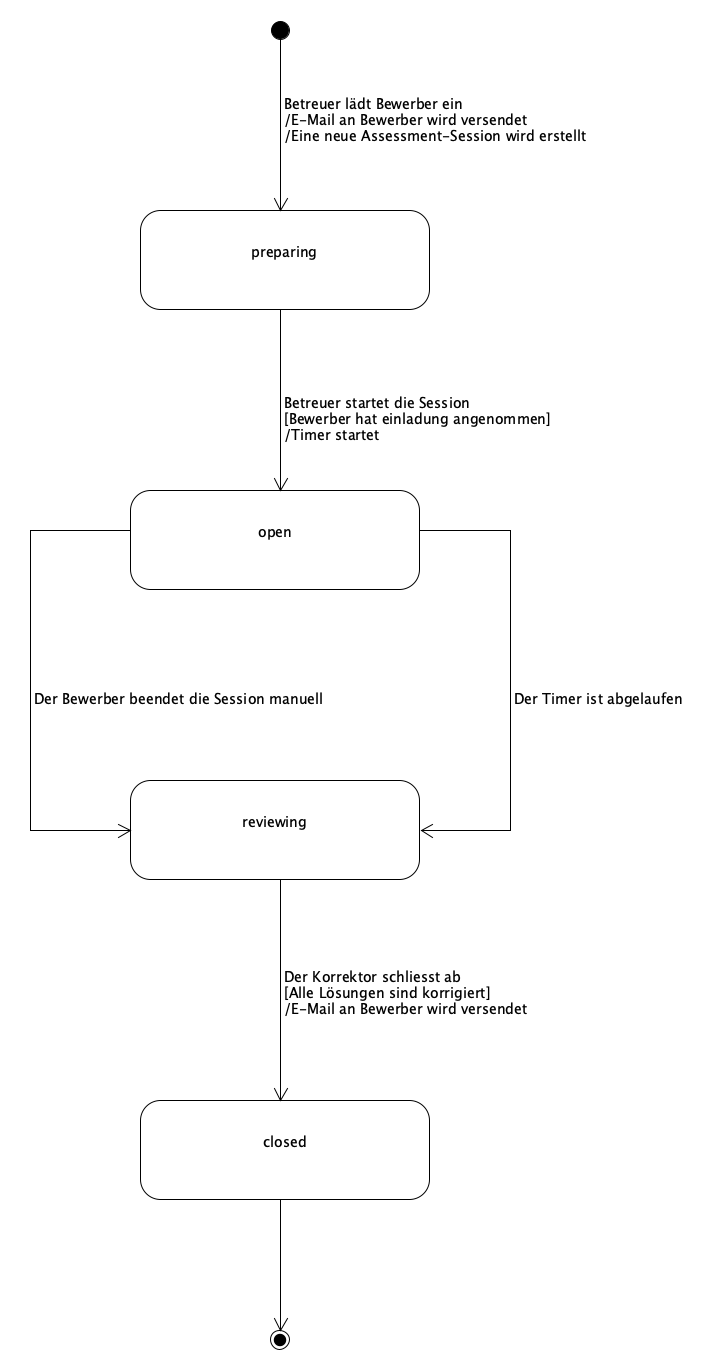
\includegraphics[height=17cm]{images/diagrams/state.png}
    \caption{\label{fig:state-diagram}Zustandsdiagramm eines Assessments nach UML 2.0}
\end{figure}

\newpage

\section{Mockups}

In diesem Abschnitt folgen grobe Entwürfe der verschiedenen Ansichten der Applikation. Diese sollen die Realisierung
erheblich vereinfachen und verschaffen nicht nur einen Überblick über das UI-Design, sondern auch über die genaueren
Funktionalitäten und Benutzer-Flows der Applikation. Die Entwürfe wurden ausserdem nach den Akteuren \ref{tab:participants} kategorisiert.

Bei den Designentwürfen wurde darauf geachtet, diese möglichst minimalistisch zu halten und strikt der Aufgabenstellung zu folgen.
Es wurden keine überflüssigen Elemente eingebaut, um sowohl die Realisierung als auch die spätere Nutzung der Applikation zu vereinfachen.

Ausserdem soll das UI, wie auch schon in den Entwürfen gezeigt wird, vorerst in Englisch umgesetzt werden, da die  offizielle Firmensprache
in der Renuo AG Englisch ist.

\subsection{Bewerber}
\begin{figure}[H]
    \centering
    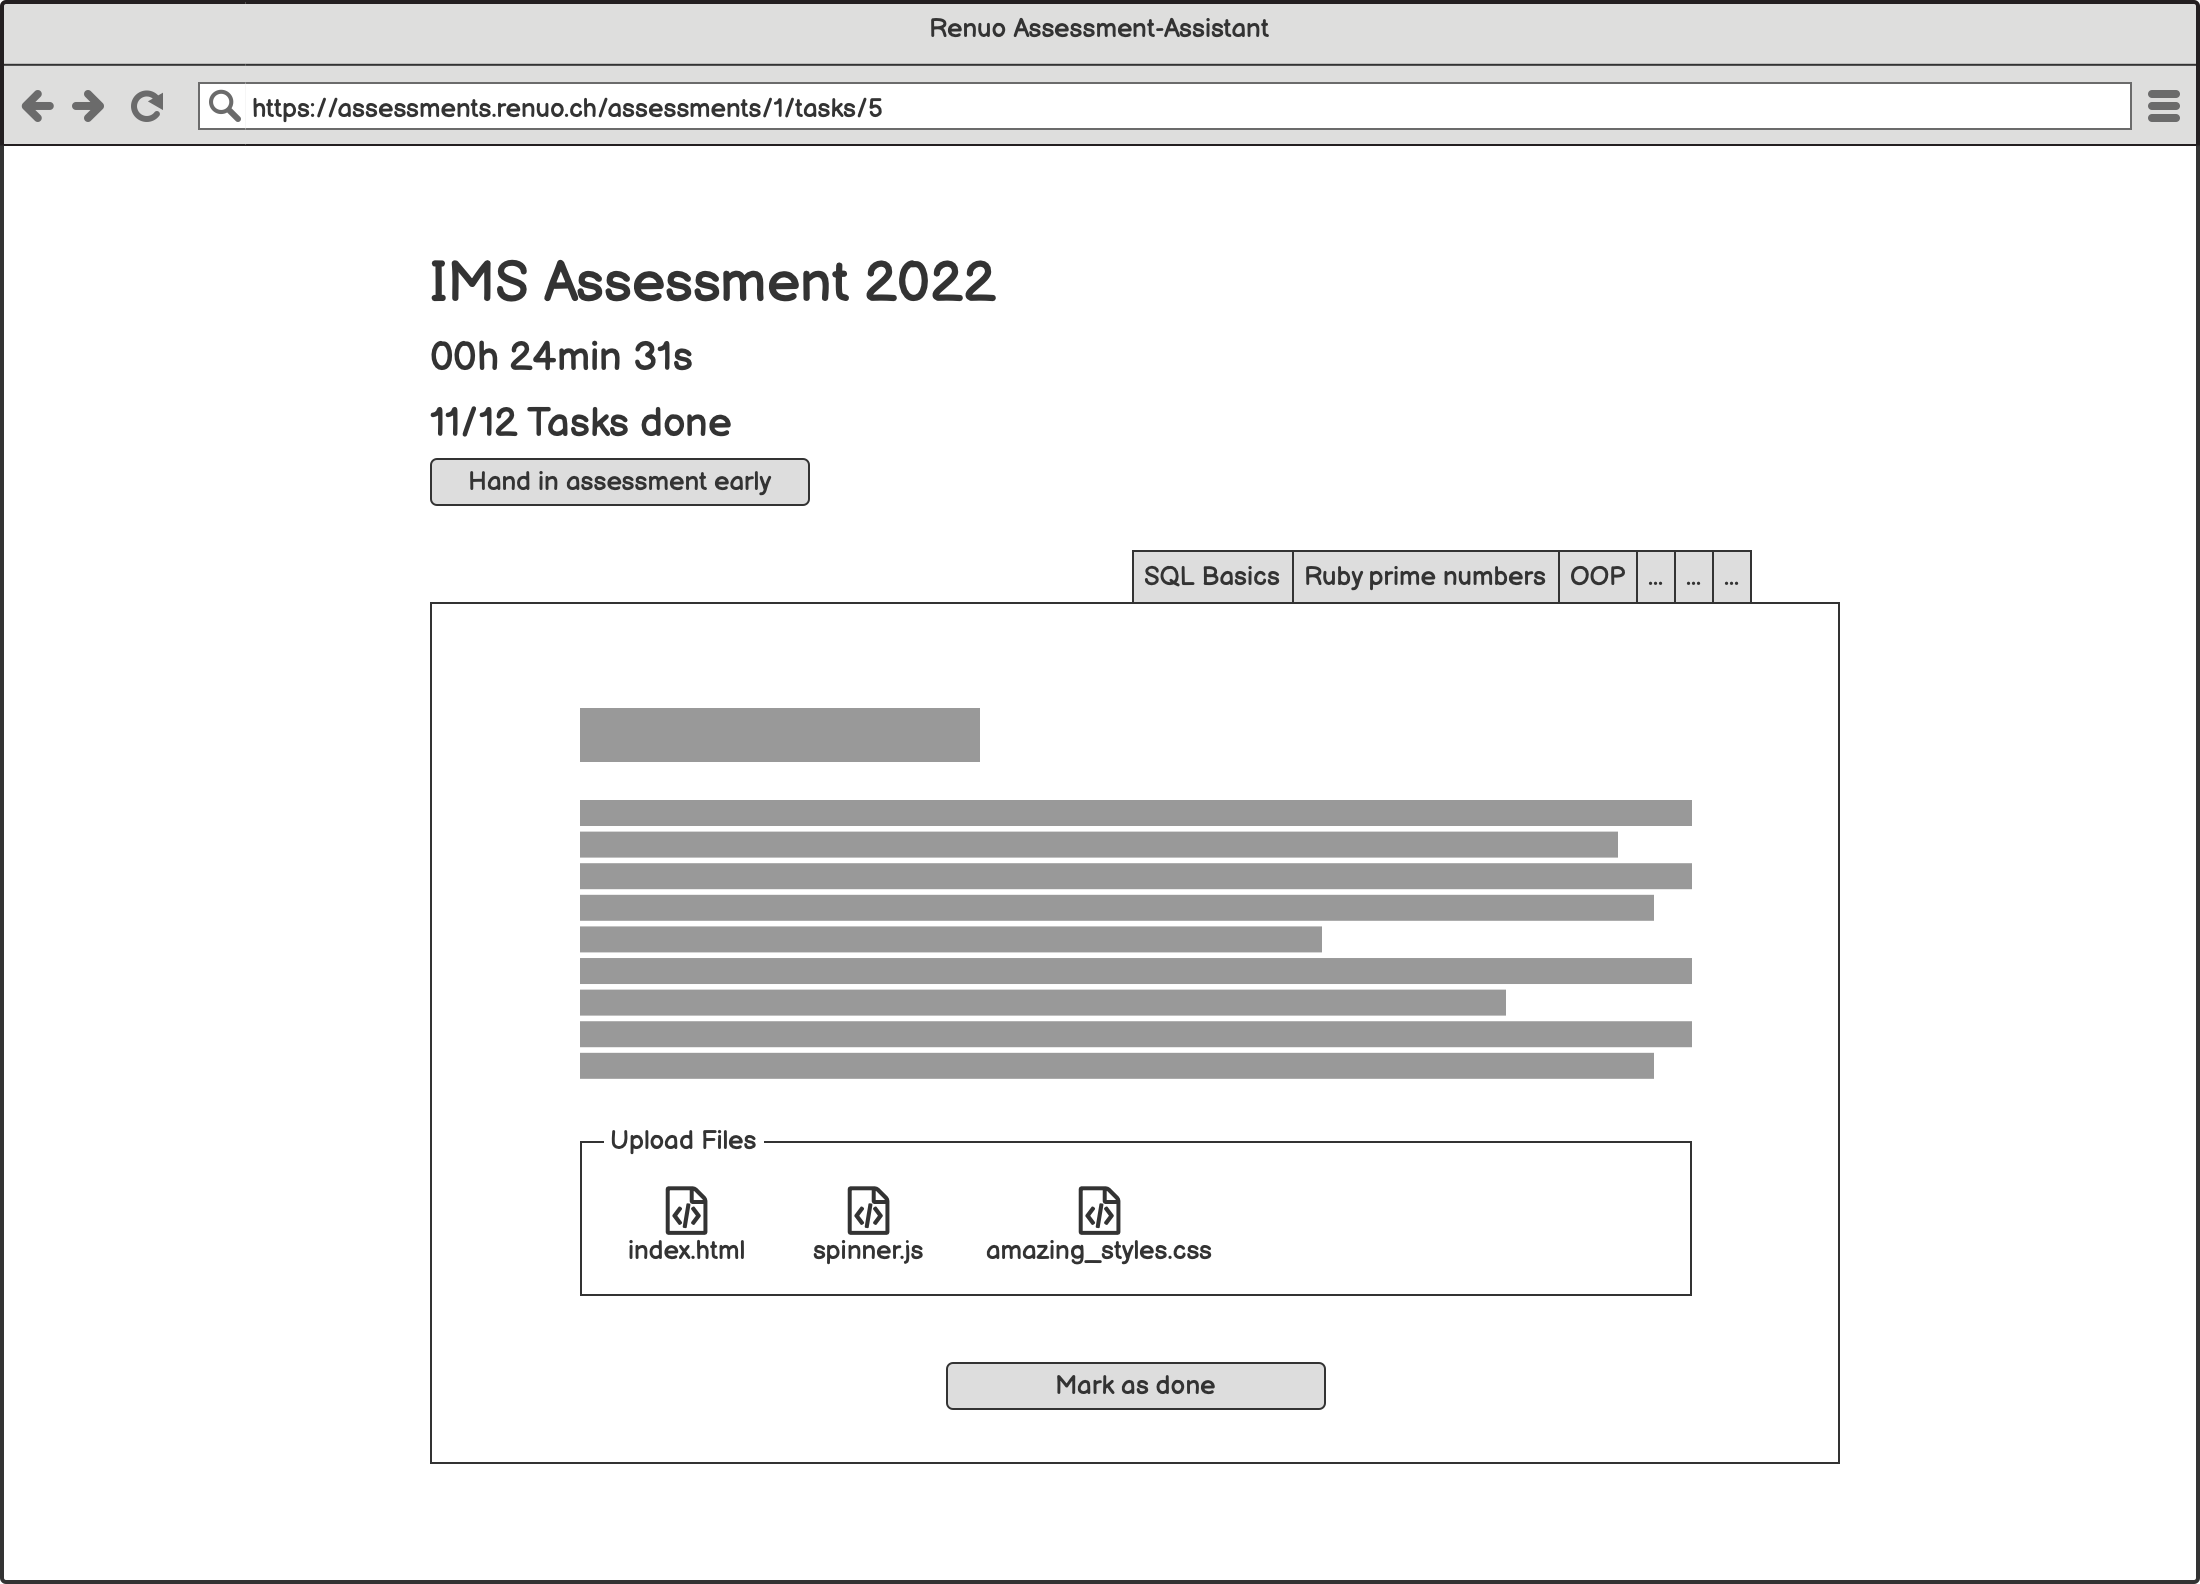
\includegraphics[width=12cm]{images/mockups/candidate-solve-assessment.png}
    \caption{\label{fig:mockup-candidate-solve-assessment}Entwurf für das Lösen eines Assessments}
\end{figure}

\subsection{Betreuer}
\begin{figure}[H]
    \centering
    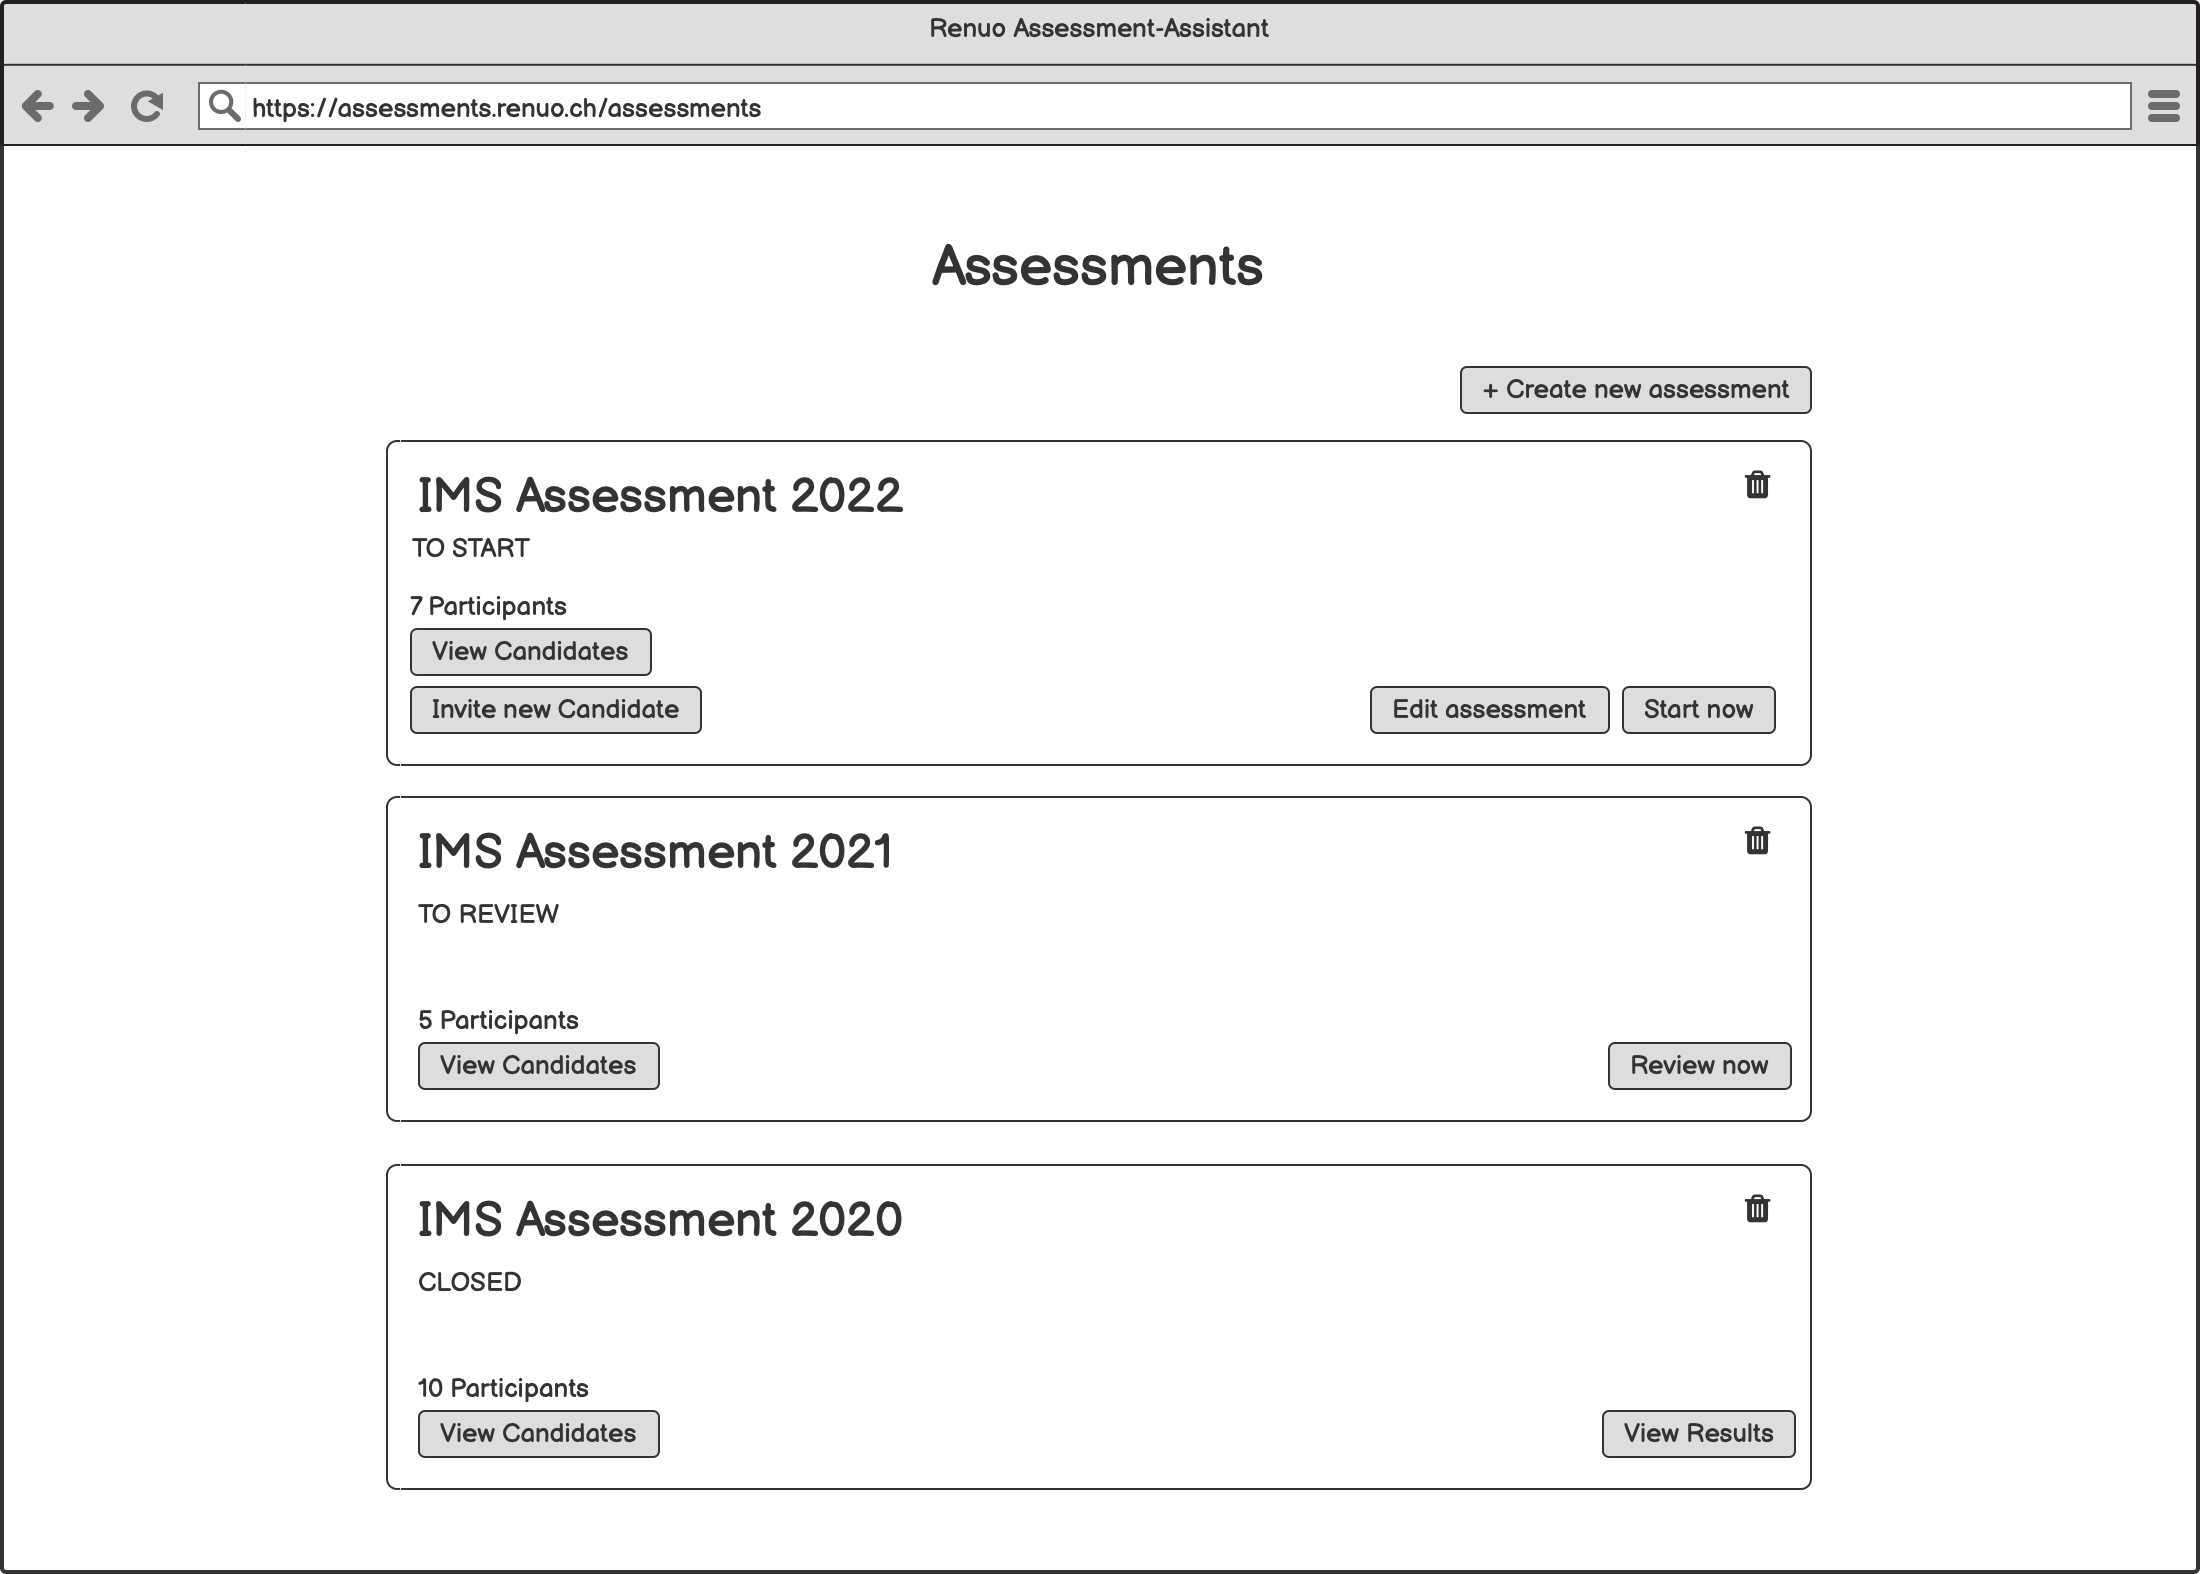
\includegraphics[width=12cm]{images/mockups/supervisor-list-assessments.png}
    \caption{\label{fig:mockup-supervisor-list-assessments}Entwurf für das Auflisten von Assessments}
\end{figure}
\begin{figure}[H]
    \centering
    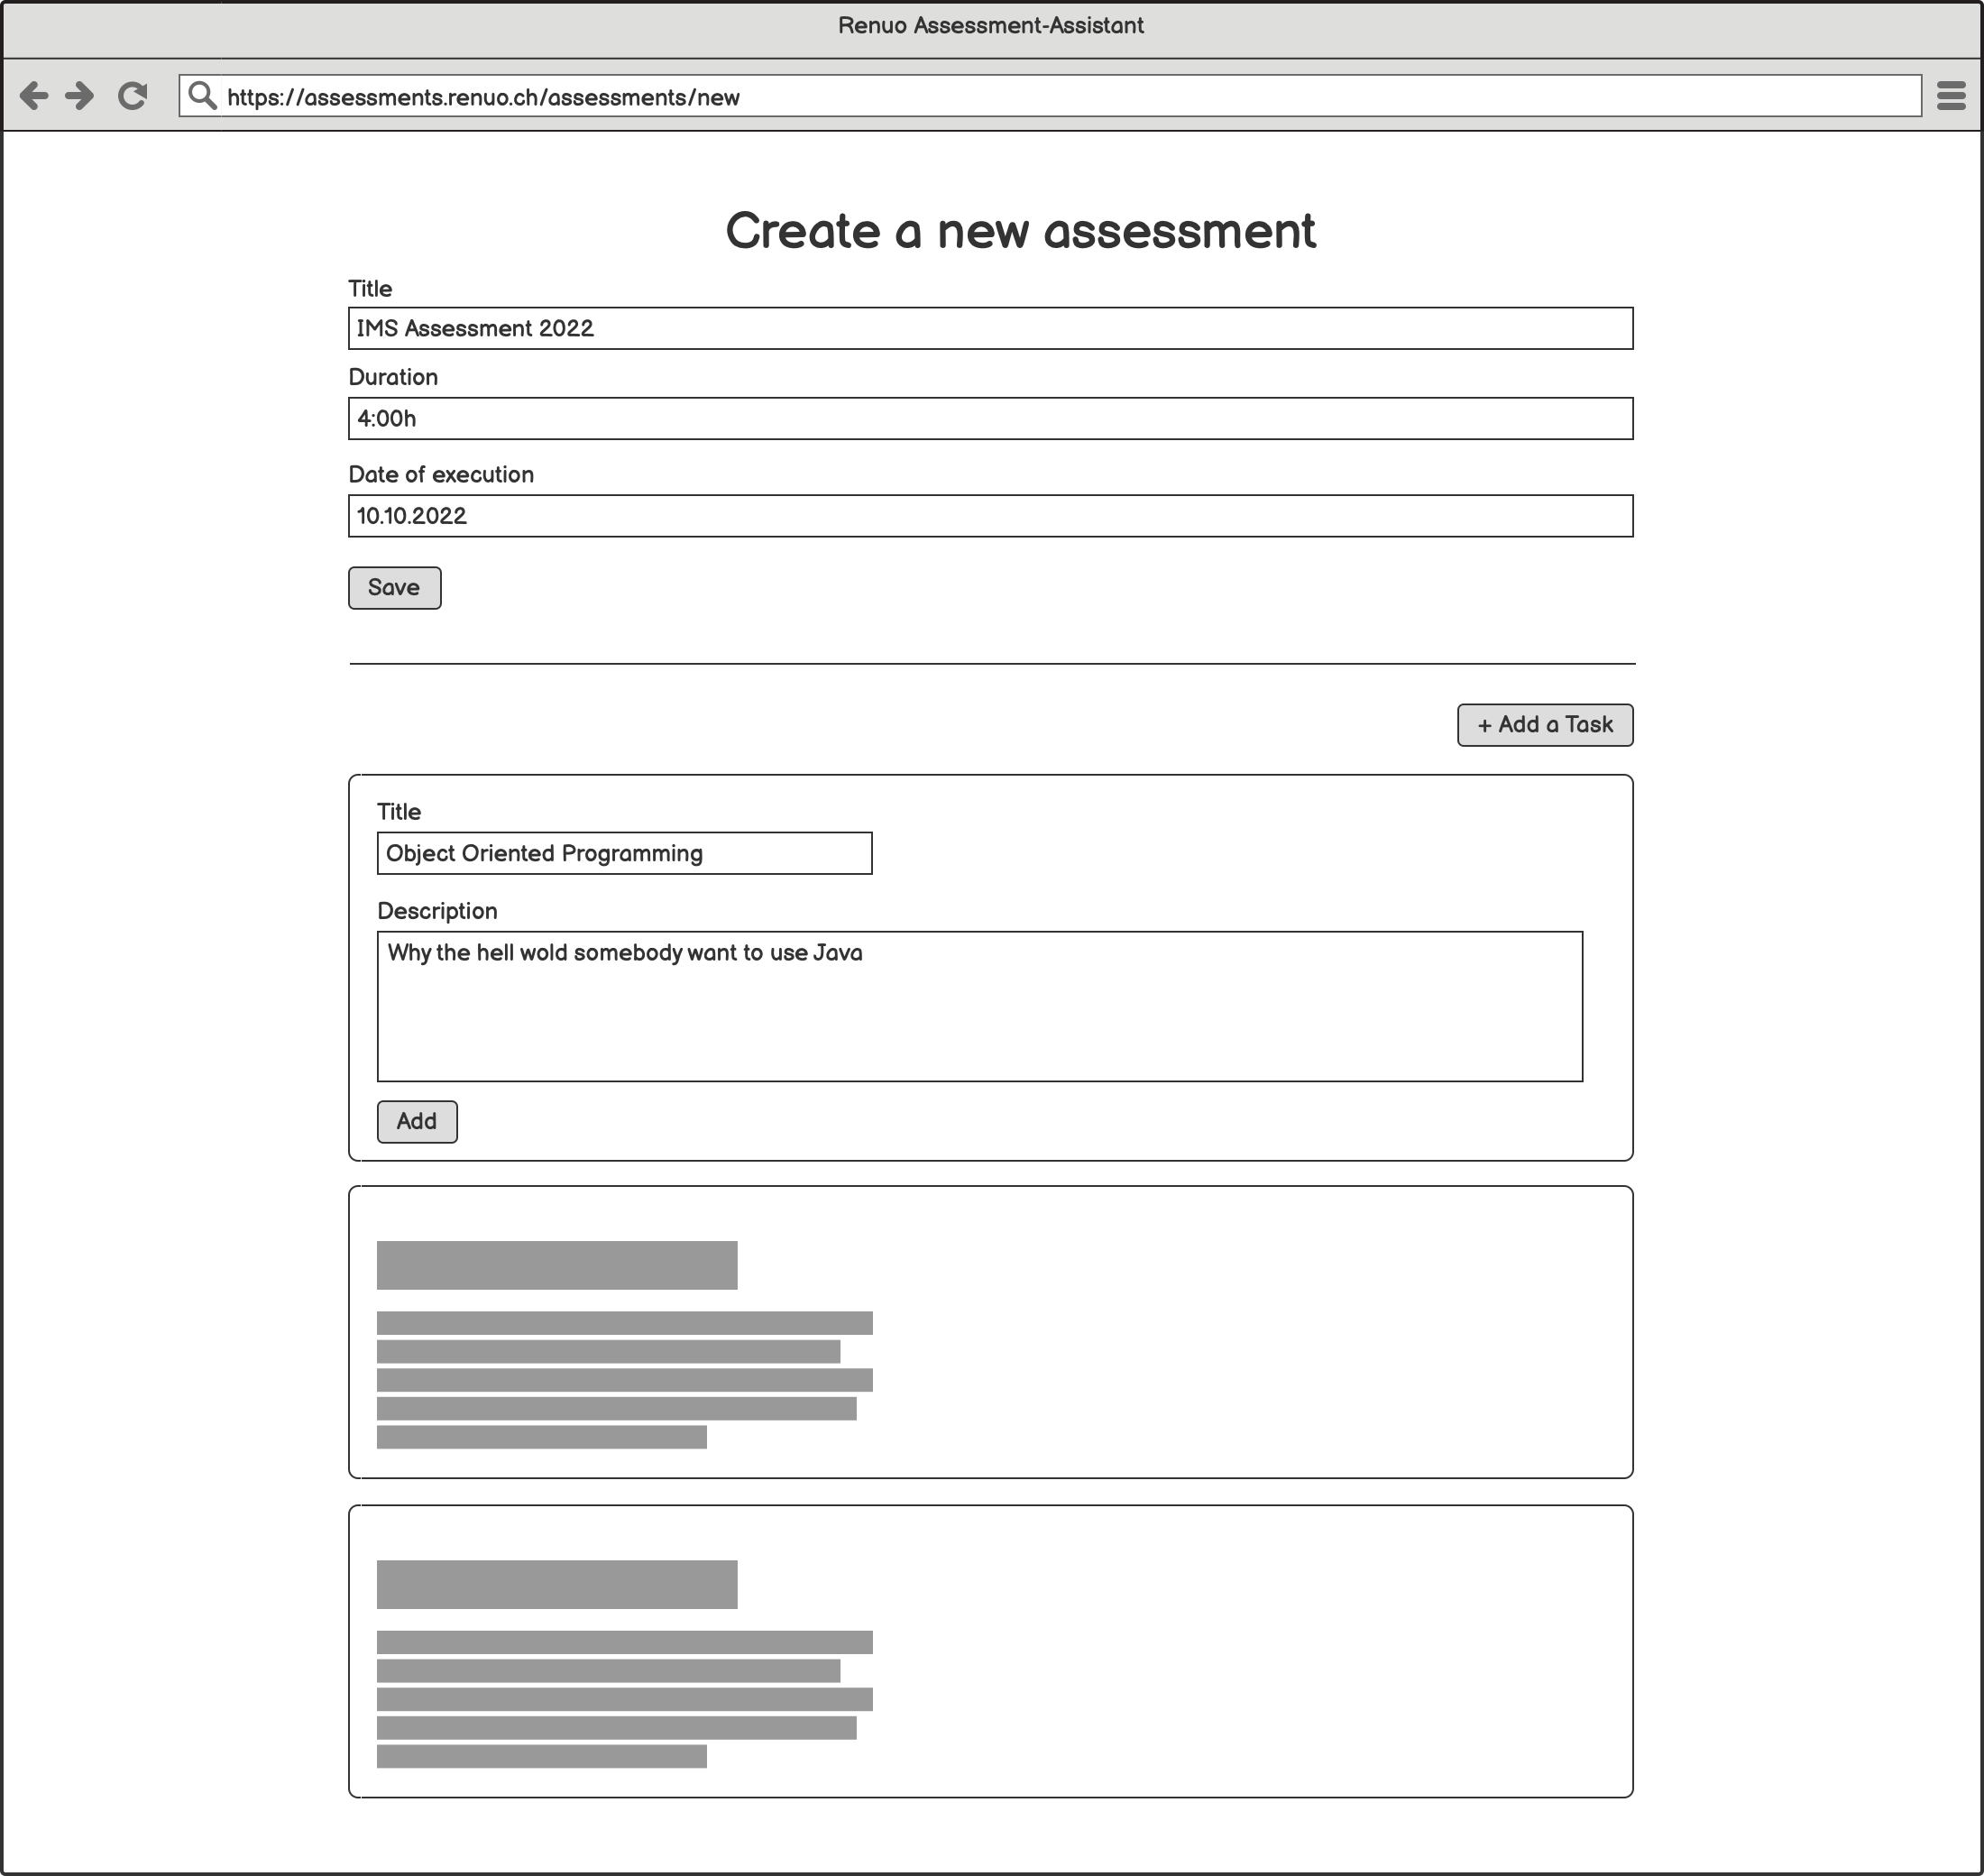
\includegraphics[width=12cm]{images/mockups/supervisor-create-assessment.png}
    \caption{\label{fig:mockup-supervisor-create-assessment}Entwurf für das Erstellen eines neuen Assessments}
\end{figure}

\subsection{Korrektor}
\begin{figure}[H]
    \centering
    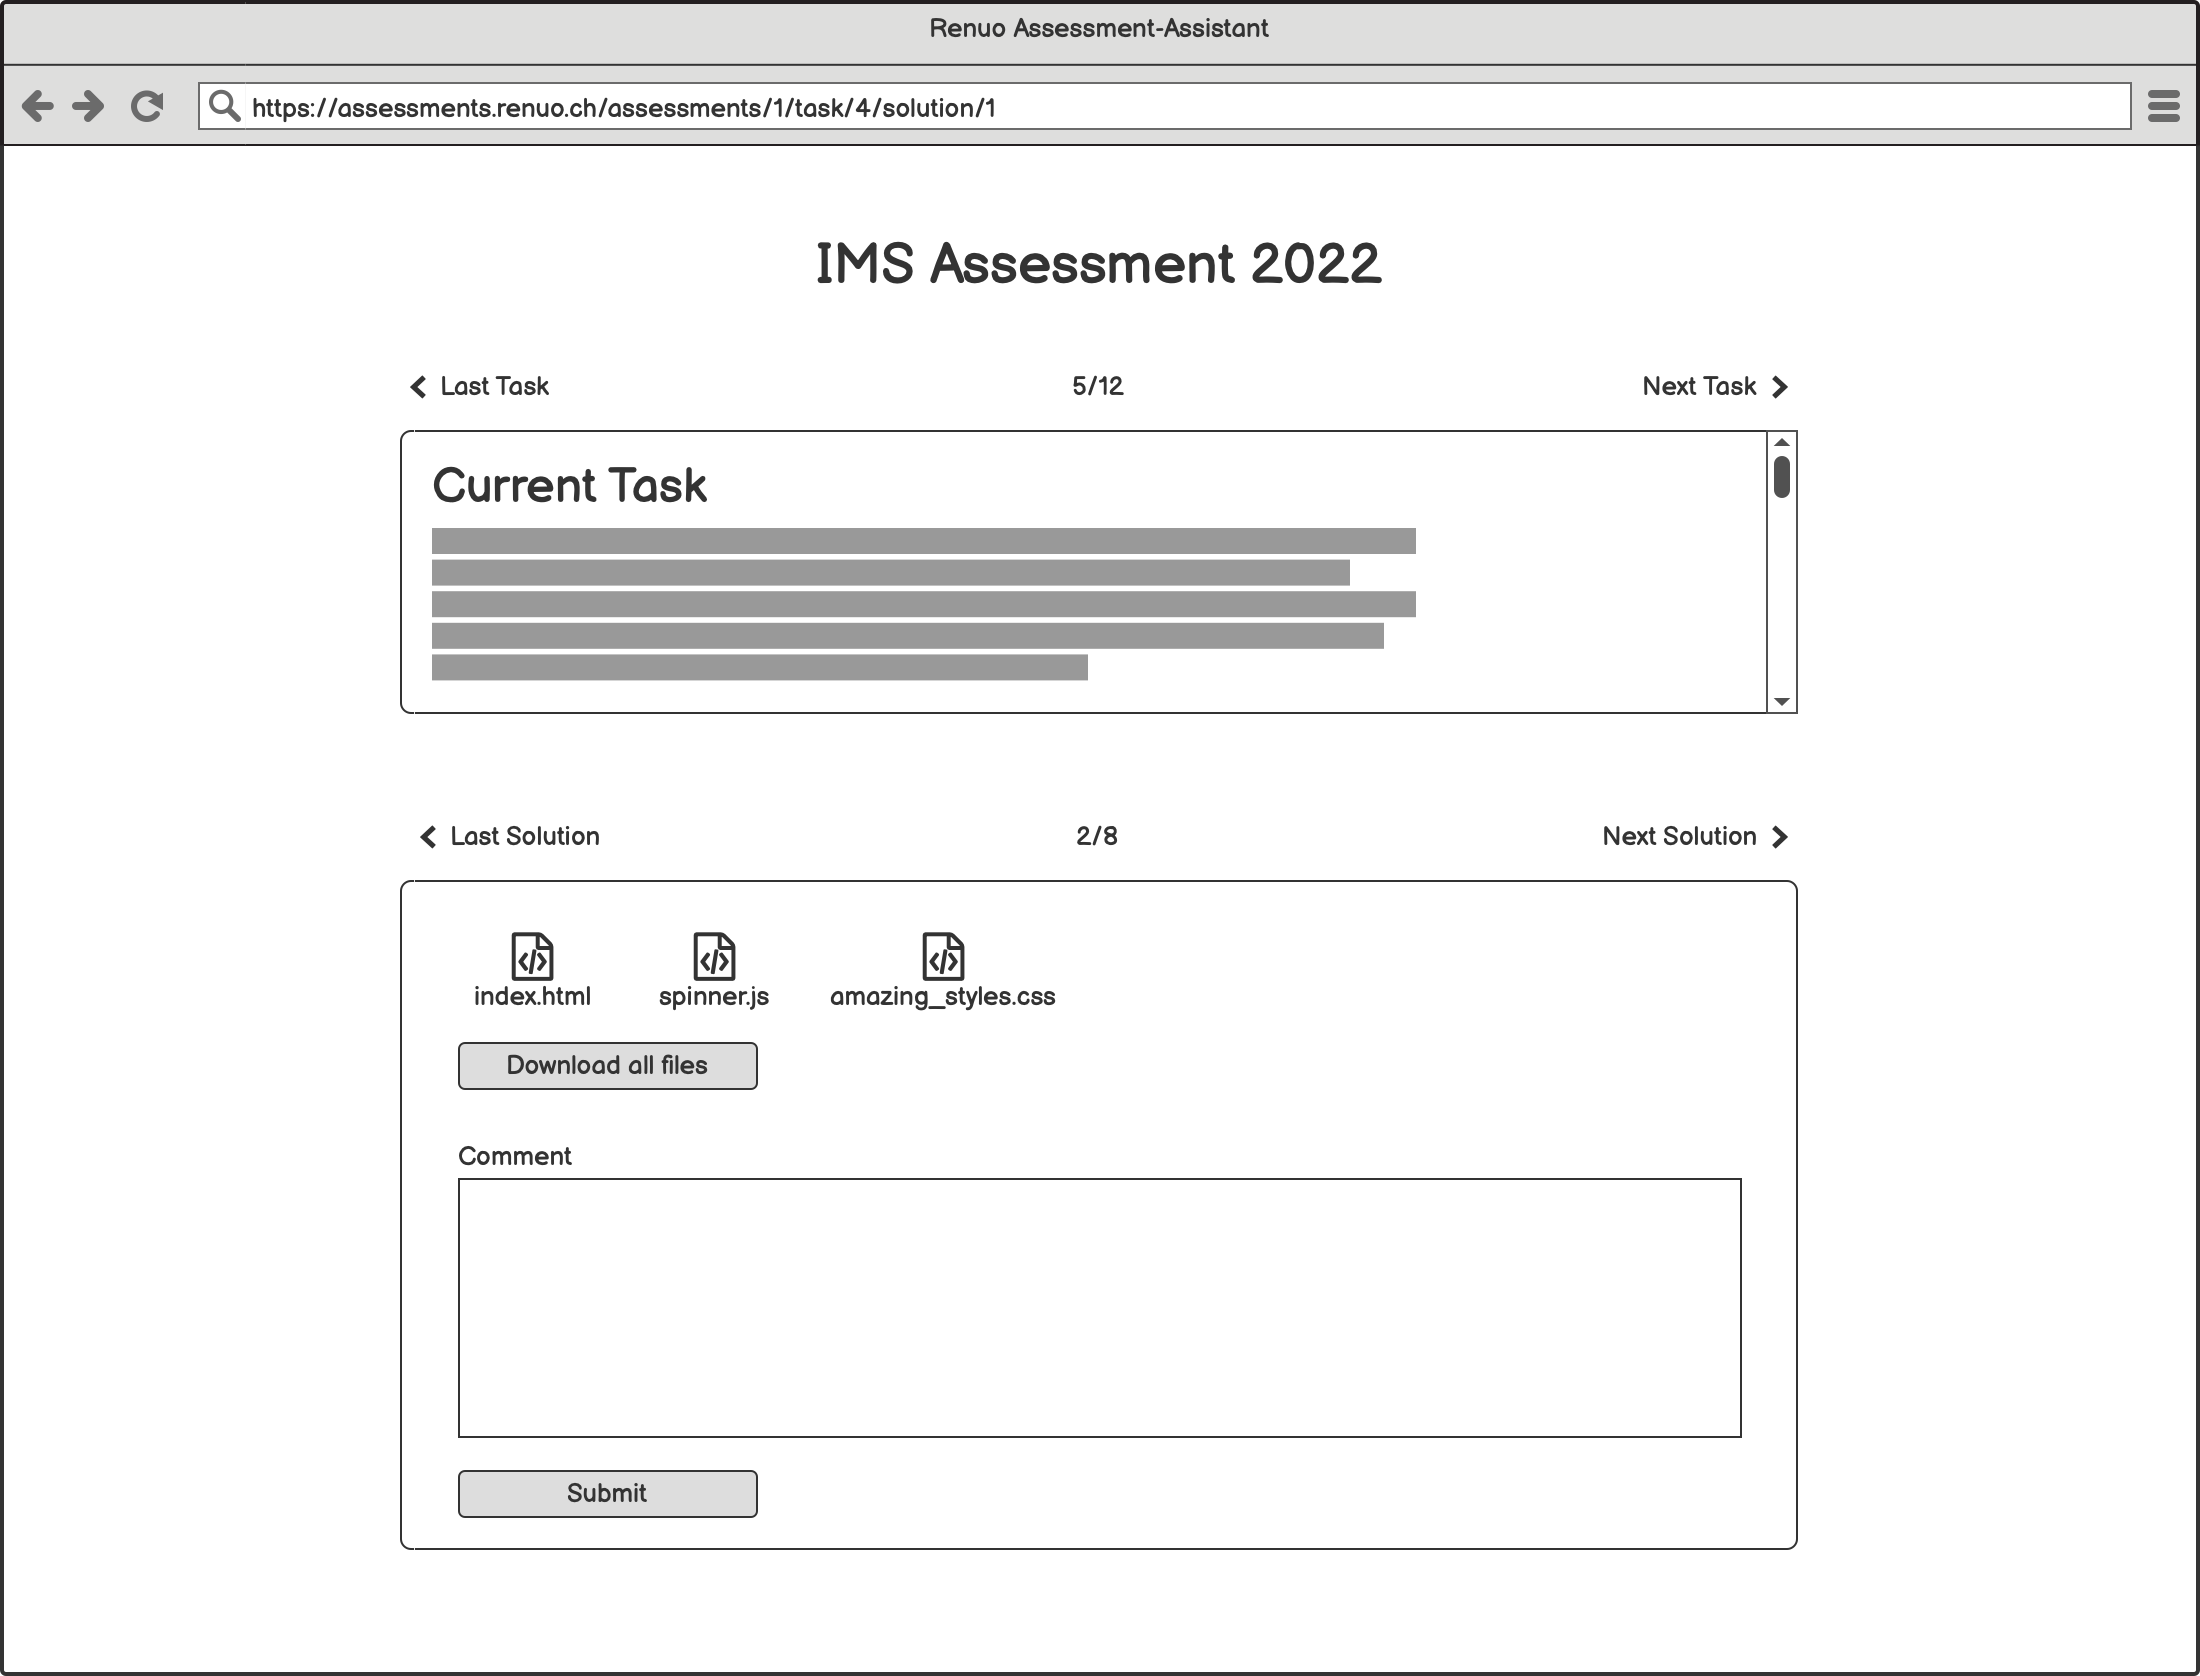
\includegraphics[width=12cm]{images/mockups/corrector-correct-assessment.png}
    \caption{\label{fig:mockup-solve-assessment}Entwurf für das Korrigieren eines Assessments}
\end{figure}
\begin{figure}[H]
    \centering
    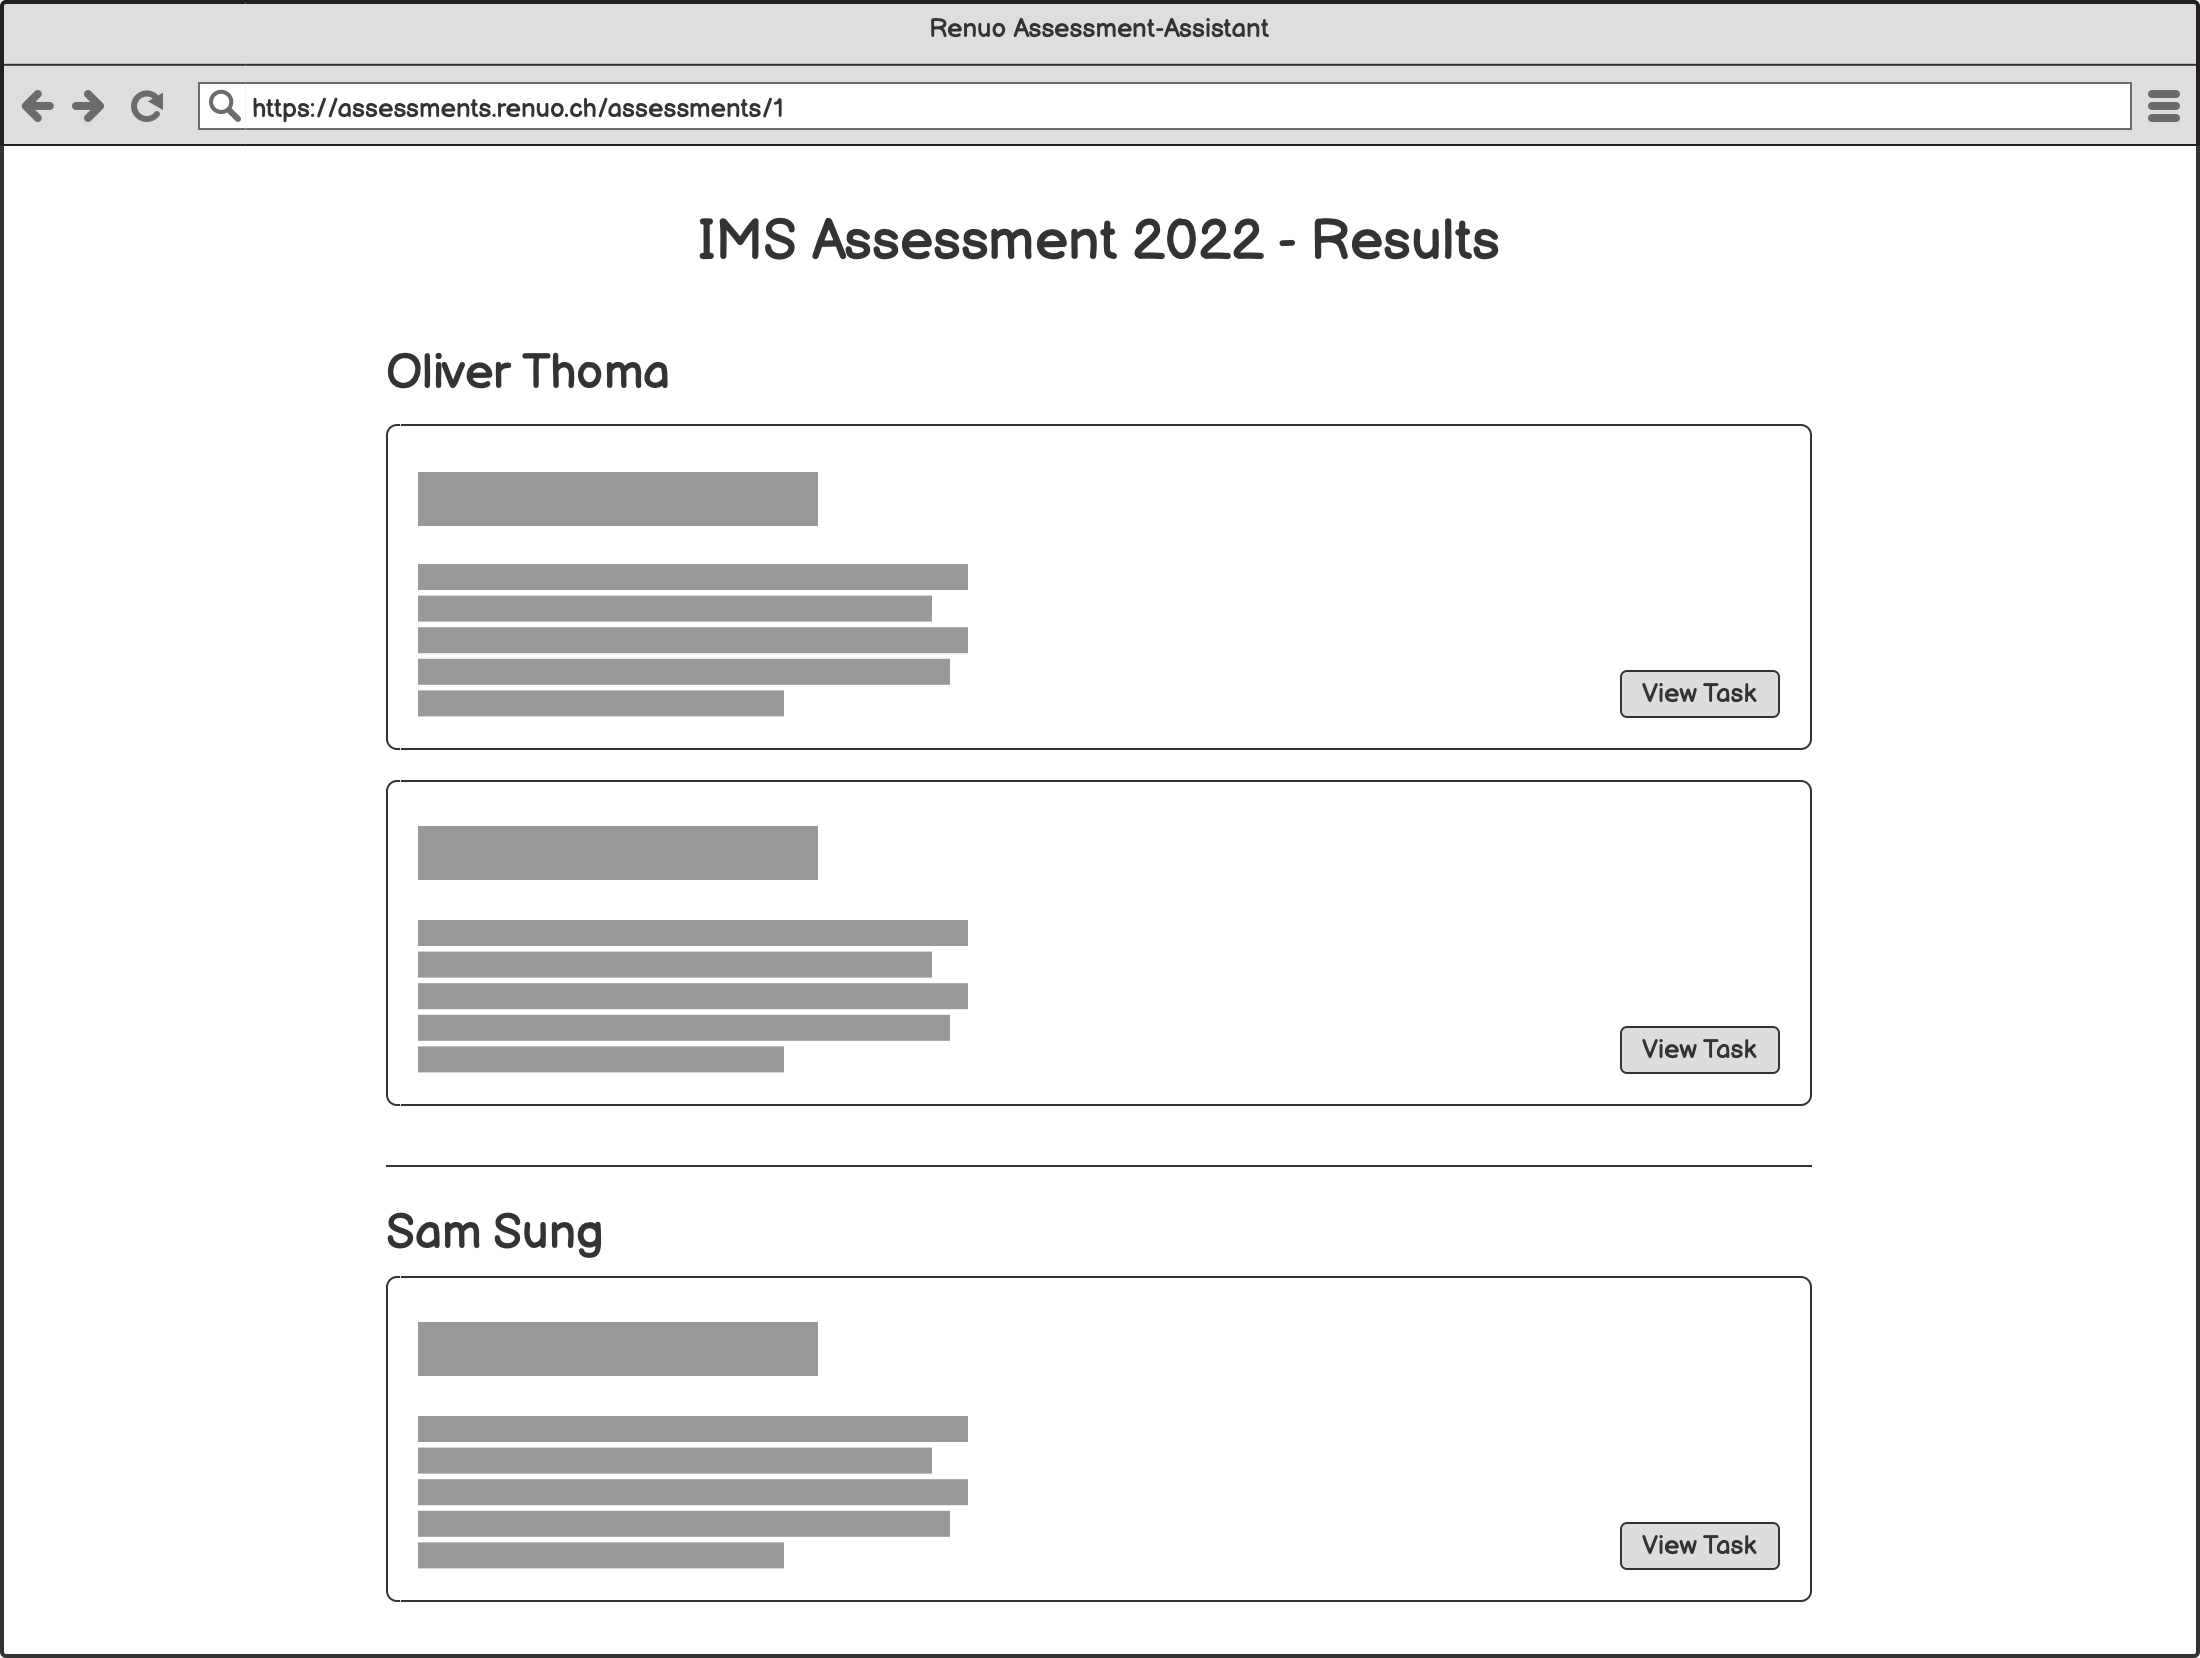
\includegraphics[width=12cm]{images/mockups/assessment-results.png}
    \caption{\label{fig:mockup-assessment-results}Entwurf für das Einsehen und Auflisten der Korrekturen}
\end{figure}

\newpage

\section{Testkonzept}

Das Testkonzept beschreibt, wie und mit welchen Werkzeugen das Resultat auf seine Richtigkeit kontrolliert wird.

\subsection{Automatisierte Tests}

Grundsätzlich wird versucht eine Testabdeckung von 100\% durch automatisierte Tests zu erreichen. Die einzelnen
Ziele/Meilensteine der Realisierungsphase werden in dieser PA testgetrieben implementiert. Das heisst, es werden zu Beginn
Unit- und Integrationstests geschrieben und erst dann wird die eigentliche Funktionalität implementiert, bis alle Tests erfolgreich durchlaufen. Dadurch wird
bereits im Voraus über die genauere Implementation nachgedacht und es garantiert immer eine vollständige Testabdeckung.

Bei jedem push auf das Git Repository wird der Code die CI/CD Pipelines auf einer modernen Linux-Umgebung durchlaufen.

Als Testmittel werden ausserdem folgende Softwarebibliotheken eingesetzt:
\begin{itemize}
    \item RSpec
    \item Capybara
    \item FactoryBot
    \item Faker
\end{itemize}

Das Framework benutzt standardmässig eine dedizierte Testdatenbank, die nach jedem Test gereinigt wird. So gibt es keine Abhängigkeiten
oder Konflikte unter einzelnen automatisierten Tests. Die zwei gems \emph{FactoryBot} und \emph{Faker} ermöglichen ausserdem möglichst
realitätsnahe und konsistente Testdaten- und Strukturen.

\subsubsection{Unit Tests}
Alle Model-, Helper- und Service-Klassen werden mittels RSpec Unit-Tests getestet. Diese sollen überprüfen,
ob die einzelnen Komponenten so Arbeiten, wie diese es beabsichtigen.

\subsubsection{Integration Tests}
Die Controller werden per RSpec Integration-Tests getestet. So werden alle Komponenten im Stack der Applikation von ganz oben
nach ganz unten getestet und es wird eine korrekte Integration der darunterliegenden Komponenten sichergestellt.

\subsubsection{System Tests}
Für die einzelnen Benutzer-Flows aller Akteure werden System Tests mit Capybara geschrieben.
Diese öffnen einen headless Chromium Webbrowser und klicken sich automatisiert durch eine im Voraus definierte Sequenz durch.
Dabei werden keine Sonderfälle, sondern lediglich die Happy-Paths getestet, da die restlichen Sonderfälle wie z.B. Validierungen bereits durch andere Tests gedeckt sind.

\newpage

\subsection{Manuelle Tests}

Die automatisierten Tests decken bereits die wichtigsten Funktionalitäten ab,
jedoch gibt es dennoch Teile in der Applikation, die nur im Kontext des Gesamtsystems getestet werden können.

Die folgenden Tests sollen demnach die vollständige und korrekte Integration der Ruby on Rails Applikation in die Produktions-Umgebung sicherstellen.
Diese werden manuell in einem Web-Browser auf der lokalen Umgebung des Kandidaten ausgeführt, welche in \ref{sec:tools} beschrieben wird.

\subsubsection{Integration von ActiveStorage mit Amazon S3}
\begin{tabularx}{\textwidth}[H]{|s|X|}
    \hline
    ID                  & 1 \\
    \hline

    Beschreibung        &
    Upload und Download von Dateien in realistischen Grössen (etwa 250MB) funktionieren ordnungsgemäss
    \\ \hline

    Vorraussetzung      &
    \begin{itemize}
        \item Einige geeignete Dateien für den Upload wurden vorbereitet
        \item Ein Assessment wurde für diesen Test erstellt und ein Bewerber wurde eingeladen
        \item Man ist eingeloggt mit einem \enquote{Bewerber} Account
    \end{itemize}
    \\ \hline

    Schritte            &
    \begin{itemize}
        \item Das Assessment, zu dem der Bewerber eingeladen wurde, starten und öffnen
        \item Im ersten Task die Datei hochladen
        \item Das Assessment frühzeitig abgeben
        \item Ausloggen und mit einem \enquote{Korrektor} Account einloggen
        \item In die Korrekturansicht wechseln und die Datei herunterladen
    \end{itemize}
    \\ \hline

    Erwartetes Ergebnis &
    Der Bewerber kann die Datei problemlos hochladen und der Korrektor kann diese im ganzen Umfang herunterladen und einsehen.
    \\ \hline
\end{tabularx}

\subsubsection{Integration mit dem Sparkpost E-Mail Service}
\begin{tabularx}{\textwidth}[H]{|s|X|}
    \hline
    ID                  & 2 \\
    \hline

    Beschreibung        &
    E-Mail Benachrichtigungen werden versendet
    \\ \hline

    Vorraussetzung      &
    \begin{itemize}
        \item Es besteht eine E-Mail-Adresse, auf die man Zugriff hat
        \item Es besteht ein \enquote{Betreuer} Account, mit dem bereits ein Assessment für diesen Test erstellt wurde
        \item Man ist eingeloggt mit einem \enquote{Betreuer} Account
    \end{itemize}
    \\ \hline

    Schritte            &
    \begin{itemize}
        \item Auf die Übersichtsseite der Assessments navigieren
        \item Einen neuen Bewerber zu diesem Assessment einladen - mit der vorbereiteten E-Mail-Adresse
    \end{itemize}
    \\ \hline

    Erwartetes Ergebnis &
    Der Bewerber erhält eine Benachrichtigung in sein E-Mail-Postfach, dass er zu einem Assessment bei der Renuo AG eingeladen wurde.
    \\ \hline
\end{tabularx}

\subsubsection{Integration von Hintergrundprozessen mit Heroku-Redis}
\begin{tabularx}{\textwidth}[H]{|s|X|}
    \hline
    ID                  & 3                                                                                        \\
    \hline

    Beschreibung        &
    Der Hintergrundprozess für das rechtzeitige Beenden eines Assessments wird korrekt ausgeführt
    \\ \hline

    Vorraussetzung      &
    \begin{itemize}
        \item Es besteht ein \enquote{Betreuer} Account, mit dem bereits ein Assessment für diesen Test erstellt wurde.
              Dabei sollte die Zeit des Assessments relativ niedrig gesetzt werden.
        \item Es besteht ein \enquote{Bewerber} Account, der bereits in das Assessment eingeladen wurde.
    \end{itemize} \\ \hline

    Schritte            &
    \begin{itemize}
        \item Das Assessment manuell über den \enquote{Betreuer} Account starten.
        \item Mit \enquote{Bewerber} Account einloggen und auf die Aufgabenübersicht wechseln. Dort bleiben, bis der Timer abläuft.
    \end{itemize}
    \\ \hline

    Erwartetes Ergebnis &
    Ein Beenden des Assessments wird nach Ablauf der Zeit erzwungen und dessen Status ändert sich zu \enquote{Reviewing}.
    \\ \hline
\end{tabularx}
